\section{Fixed workflows}
\label{sec:fixed}

The architectures in these notes differ in which decisions about a run the designer makes before it
starts and which are made while it runs (\cref{sec:agents}). The first one we study, the fixed
workflow, leaves every decision about how a run proceeds to the designer, who makes them before the
program runs. In exchange, the program gains guarantees that the later architectures give up,
which makes the fixed workflow the baseline for comparing them. We explain the idea with
\msa{}, the course's running example, and then examine Agentless, a published system built the
same way.

\subsection{What a fixed workflow is}
\label{sec:fixed-definition}

A \textbf{fixed workflow} is a program whose steps, and their order, are decided by the designer
before any task arrives. A \textbf{step}, also called an operation, is one unit of work the program
performs, such as reading lines of a file, calling the model once, or submitting a patch. The model
is still called, but only to produce content at points the designer has chosen, for example to
rank candidate files or to write a patch. It never decides what the program does next.

A run is one execution of the program on one task (\cref{sec:agents-msa}), which in our running
example is one scanner alert. It helps to separate two kinds of decisions about a run. \textbf{Control decisions}
determine how the run proceeds. \textbf{Content decisions} determine what each step produces, such
as which file to patch and what the patch says. The control decisions cover four things:
\bi
\item \textbf{Operations.} The designer decides which step runs next, and whether any step follows
it.
\item \textbf{Model calls.} The designer decides how many times the run calls the model.
\item \textbf{Termination.} The designer decides what ends the run.
\item \textbf{Artifacts.} The designer decides which artifacts each step reads and writes. An
\textbf{artifact} is a named output of one step that a later step can read, such as a list of
candidate lines or a patch.
\ei

A decision is made at \textbf{design time} when we, as the designer, make it while writing the
program, before any task arrives. It is made at \textbf{run time} when the program, or the model it
calls, makes it during a run. In a fixed workflow, we make every control decision at design time,
and the model makes content decisions at run time. No output of the model can change a control
decision.

In our running example, \msa{} receives one scanner alert that flags a line of code, and its task
is to patch that code. A fixed workflow for this task could consist of four steps: read the region
around the flagged line, ask the model to name the lines to edit, ask the model to write the patch,
and submit the patch to a fixed set of checks that accept or reject it. Every alert goes through
the same steps, once each, in the same order. We refer to this fixed-workflow version of \msa{} as
\textbf{the chain}, because its steps run one after another in a sequence set in advance.

\subsection{Who decides, and when}
\label{sec:fixed-decisions}

Every decision in a fixed workflow has an owner and a time at which it is made
(\cref{tab:fixed-decisions}). In the table, ``Us'' means the designer. The rows above the heavy
rule are control decisions, which we make at design time. The rows below it are content decisions,
which the model makes at run time.

\begin{table}[htbp]
  \caption{Decisions in a fixed workflow, with who makes each one and when. The heavy rule separates
  the control decisions, made by the designer, from the content decisions, made by the model.}
  \label{tab:fixed-decisions}
  \begin{adjustbox}{width=\linewidth}\begin{tabularx}{\linewidth}{XL{0.23\linewidth}L{0.2\linewidth}}
    \toprule
    \textbf{Decision} & \textbf{Who decides} & \textbf{When} \\
    \midrule
    \textbf{Which operation runs next} & Us & Design time \\
    \textbf{Whether anything runs after it} & Us & Design time \\
    \textbf{How many model calls the run makes} & Us & Design time \\
    \textbf{What ends the run} & Us & Design time \\
    \midrule[\heavyrulewidth]
    \textbf{What a model call returns} & The model & Run time \\
    \textbf{Which values travel to the next step} & The model & Run time \\
    \bottomrule
  \end{tabularx}\end{adjustbox}
\end{table}

Both of the model's decisions concern values. The model decides what a call returns, for example
the text of a patch. It also decides which values travel to the next step, for example which
candidate files it ranks highest and therefore which files the next step receives. This does not
conflict with the designer's control over artifacts. The designer decides that the next step reads
the artifact holding the ranked files. The model decides which files that artifact contains.

This division is about authority, not difficulty. Choosing the right file to patch is often the
hardest part of the task, and it is left to the model. The designer keeps a comparatively easy
decision, the order of the steps, for example that a file is chosen before its lines are read.
That decision carries the authority over what happens next.

A fixed workflow need not be a straight line of steps. It may branch, filter a set of candidates,
or repeat a step a set number of times. A \textbf{predicate} is the condition in the code that
selects a branch. The workflow remains fixed because we wrote every predicate it tests and we set
every number of repetitions.

Which branch a particular run takes can depend on data produced during the run, such as which
candidate patches pass the tests. The set of possible paths cannot, so we can list every path
before the program runs. Agentless (\cref{sec:fixed-agentless}) is an example: it samples a fixed
number of candidate patches and filters them by running tests.

The model's output is treated as data. A step may store it, pass it to the next step, or write it
into a file. The program never reads it as an instruction that names the next step. This is why no
output of the model can change a control decision.

\subsection{Prior knowledge and autonomy}
\label{sec:fixed-autonomy}

A fixed workflow knows about its task only what its designer put into it. Every control decision
records an expectation we formed before any particular task was seen. In the vocabulary of
\cref{sec:agents-rational}, these decisions rely on prior knowledge, the knowledge built in by the designer.
They do not rely on the program's percepts, the information it receives during the run, such as the
contents of the files it reads.

\begin{definition}[Autonomy]
\label{def:fixed-autonomy}
``To the extent that an agent relies on the prior knowledge of its designer rather than on its own
percepts and learning processes, we say that the agent lacks autonomy.''
\citep[\S2.2.3]{russell2020aima}
\end{definition}

In its control decisions, a fixed workflow lacks autonomy in exactly this sense. What it reads
during a run can change the content of a step, for example the patch the model writes. It can
change which step comes next only through a condition that we wrote in advance, so the choice of
the next step still rests on our prior knowledge.

Relying on prior knowledge is a legitimate engineering choice when that knowledge is correct, that
is, when we know in advance which steps the task needs. Writing those steps down then gives the
guarantees of shape, address and termination (\cref{sec:fixed-guarantees}). The architectures in
the following sections rely less on the designer's prior knowledge, one decision at a time,
starting with the choice of the next action (\cref{sec:reactive}).

\subsection{What a fixed workflow guarantees}
\label{sec:fixed-guarantees}

Fixing the control decisions gives three guarantees, called shape, address and termination. Each
one follows from the fact that the designer, and not the model, decides how the run proceeds.
\bi
\item \textbf{Shape.} The number and order of model calls are known before the run, because they
are the calls we wrote. The number of calls does not depend on what the model says. We can
therefore estimate the cost of a task before its run starts, and the cost of a thousand alerts
before running any of them. In the chain, every alert makes the same two model calls, whatever the
alert says.
\item \textbf{Address.} A wrong result can be traced to the step that produced it, because each
artifact is written by one step that we know in advance. The name reflects this: every failure has
a location in the program. Debugging a bad patch in the chain means reading its four artifacts in
order: the excerpt it read, the lines the model named, the patch the model wrote and the results of
the checks. It does not require reconstructing a long sequence of choices made by the model, such
as the sequence of up to forty model calls that a reactive loop can make (\cref{sec:reactive-stops}).
\item \textbf{Termination.} The run ends when its last step returns. Stopping does not depend on
anything the model says, because the last step is fixed before the run starts. The chain ends when
its submit step returns.
\ei

Each guarantee is a property of the program we have designed. None of them is a prediction about
what the model will do. The shape guarantee, for example, tells us how many calls a run makes. It
says nothing about whether the resulting patch is correct.

Termination is the guarantee that the later architectures never regain. A reactive loop, a planner
and a validator all let the model choose further steps, so the program no longer has a last step
that is known before the run. These architectures replace termination with a budget, the limit on
the number of model calls a run may make (\cref{sec:agents-not-rational}). A budget guarantees that the run stops. It does
not guarantee that the run finishes, that is, reaches an accepted submission before the budget is
spent.

In more autonomous agents, these guarantees no longer follow from the structure of the program.
Where we need one, we have to add a mechanism that provides it, as a budget on model calls provides
stopping.

\subsection{Fixed parts and open parts}
\label{sec:fixed-parts}

\begin{figure*}[t]
  \centering
  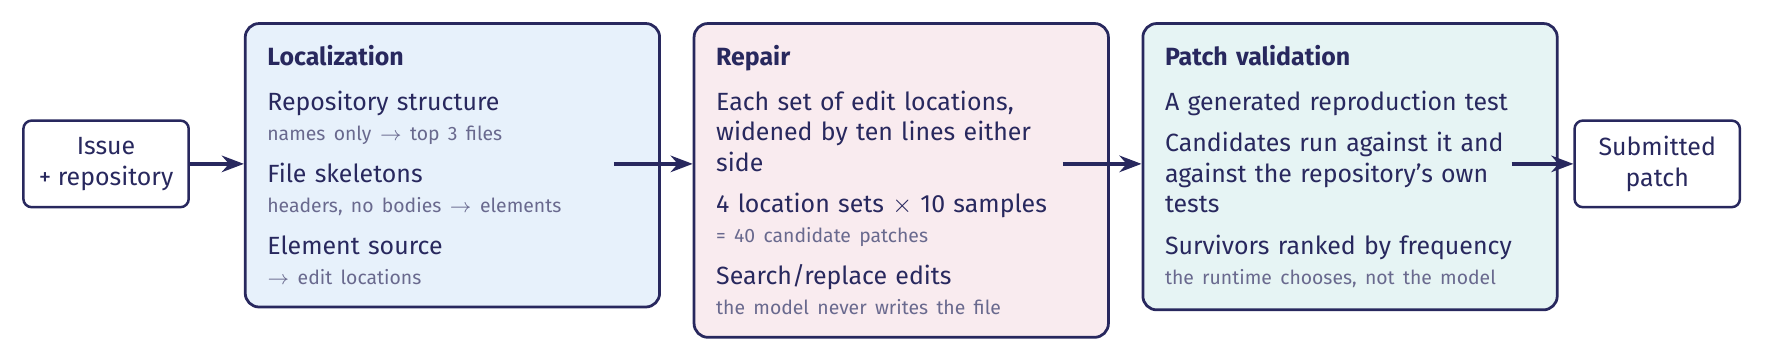
\includegraphics[width=\textwidth]{figures/deck/agentless-phases.png}
  \caption{The three phases of Agentless, run in a fixed order from an issue and its repository to
  a submitted patch. The model supplies content within each phase, but no output of the model can
  change the order of the phases. Redrawn after Figure~1 of Xia et al., FSE 2025.}
  \label{fig:fixed-agentless}
\end{figure*}

Most systems we build are partly fixed and partly open, and where the boundary falls is a design
decision. We divide a system into \textbf{stages}, each a group of steps that produces a defined
result for the next stage. A \textbf{fixed stage} makes all its control decisions at design time,
as a fixed workflow does. An \textbf{open stage} lets the model decide what runs next, as the
architectures of the following sections do.

The course's first homework, HW1, shows this division. It asks for a triage application for scanner
alerts. The application's intake stage, which produces the alerts the application will
investigate, is a fixed workflow. Its investigation loop, in which the model chooses the next step,
is an open stage.

Knowing which stages are fixed matters because budgeting, recovery, transactions and parallel
execution are all easier to engineer in a fixed stage:
\bi
\item \textbf{Budget.} We can estimate the cost of a fixed stage before it runs, because we chose
how many model calls it makes. For an open stage we can only reserve an amount and enforce a limit,
because the number of calls depends on the model's choices.
\item \textbf{Recover.} A \textbf{checkpoint} saves a run's progress so that a failed run can resume
from that point instead of starting over. A checkpoint needs named artifacts to save and to resume
from. A fixed stage names its artifacts before the run, and its boundary with the next stage is
where it hands on its defined result, so that boundary is a natural checkpoint.
\item \textbf{Transact.} A \textbf{transaction} groups a set of changes so that either all of them
take effect (a commit) or none of them do (a rollback). To decide where to commit and what to roll
back, we must know the sequence of steps in advance.
\item \textbf{Run in parallel.} Two stages can safely run at the same time only if neither one
writes what the other reads or writes. A fixed stage declares in advance which artifacts it reads
and writes, so this can be checked before the run.
\ei
In an open stage each of these is harder, because the steps and their artifacts are not known until
the run happens. The architectures in the rest of these notes pay this cost.

\subsection{What a fixed workflow gives up}
\label{sec:fixed-costs}

A fixed workflow pays for its guarantees with its ability to respond to what a run discovers.
Because every step and every branch was written before the task arrived, the program can respond to
new evidence only in the ways the designer foresaw. It cannot take a step the designer did not
write. In particular, it cannot look again, notice what is missing, or ask for more:
\bi
\item \textbf{No second look.} Every read is scheduled before we know what the first read returns,
so no read can be chosen in response to an earlier one.
\item \textbf{No sense of what is missing.} Nothing in the run represents evidence the program has
not read, so the program cannot tell that its information is incomplete.
\item \textbf{No way to ask.} If the fix depends on a file the alert never names, no step exists in
which the program could go and read it.
\ei

A fixed workflow chooses its steps from prior knowledge alone, so it is rational as long as that
knowledge is correct, that is, as long as the steps we wrote are the ones the task needs. When the
knowledge is wrong, the workflow stops being rational. Here \emph{rational} has the meaning given
in \cref{sec:agents-rational}: a rational agent chooses the action expected to maximize its
performance measure, given what it has perceived and what it was built to know.

Our task environment is partially observable (\cref{sec:agents-properties}), which means that the agent sees
only the parts of the code it reads. In such an environment, a rational agent must act in order to
gather information, because the evidence it needs reaches it only through its own actions. A fixed
workflow does gather information, because its steps read files. It reads them, however, on a
schedule we wrote before we knew what the reads would return.

When our prior knowledge is incomplete, a fixed workflow fails silently. A \textbf{silent failure}
is one that the system neither detects nor reports, so the run ends as if it had succeeded.

Consider an alert about a SQL query built from untrusted input, in which the untrusted value
reaches the flagged line through a helper function in a file the alert never names. The chain reads
only the region around the flagged line, so it never sees the helper. It does not stop early or
raise an error, and it does not report a gap in its evidence. It writes a patch for the code it was
given and submits it, and the checks run at submission pass.

The checks pass because they test less than the performance measure asks
(\cref{sec:agents-not-rational}). They confirm that the patch applies, that it touches the flagged
line, and that the rescan is clean. A clean rescan shows that the scanner no longer recognizes the
flagged pattern. It does not show that the untrusted value can no longer reach the query.

Nothing in the chain records what it did not read, so nothing in the run signals a problem. A fixed
workflow gathers only the evidence its designer scheduled, so a gap the designer did not foresee
stays invisible to it.

The next architecture, the reactive loop, adds the ability to look again. In a reactive loop, the
model sees each tool result and then chooses the next action, so it can decide to read the helper
(\cref{sec:reactive}).

\subsection{Agentless: a published fixed workflow}
\label{sec:fixed-agentless}

Agentless is a published system for repairing software issues, and it is a fixed workflow. It was
evaluated on \textbf{SWE-bench Lite}, a benchmark of 300 issues from open-source Python
repositories. For each issue, a system receives the issue description and the repository and must
produce a patch. The issue counts as \textbf{resolved} when the patch passes the benchmark's tests
for that issue. In its published comparison, Agentless resolved more of these issues than any
open-source agent it was compared with \citep{xia2025agentless}.

Agentless runs three phases in a fixed order (\cref{fig:fixed-agentless}). Each phase is a stage in
the sense of \cref{sec:fixed-parts}, handing a defined result to the next. The model supplies
content in every phase, and no output of the model can change the order.

The work around the model is done by the runtime (\cref{sec:agents-msa}), which here executes the
workflow: it calls the model, runs the tests and writes files. The runtime is a component of the
program, and it is distinct from run time, the period during which a run happens. The three phases
work as follows.
\bi
\item \textbf{Localization.} This phase finds where to edit, narrowing the search in three steps.
Each step gives the model a smaller input than the last. First, the model sees only the names of
the repository's files and folders and ranks the files most likely to need an edit. The runtime
combines this ranking with a similarity search that compares the issue text with pieces of the
code, and keeps the three files that rank highest across both. Next, the model
sees a \textbf{skeleton} of each file, meaning its class and function headers without their bodies,
and picks the relevant \textbf{elements}, the classes and functions to examine further. Finally, it
sees the source code of those elements alone and picks the edit locations. At every step the model
ranks and selects from what it is given. It never asks for anything else.
\item \textbf{Repair.} This phase writes candidate patches. Localization supplies four alternative
sets of edit locations rather than a single one. Each set is widened by ten lines on either side, so
the model sees the surrounding code, and the model samples ten patches for each set, forty
candidate patches in all. Each patch is a \textbf{search/replace edit}: the model returns a block of
code to find and a block to replace it with. The runtime, and not the model, then writes the change
to the file.
\item \textbf{Patch validation.} This phase chooses one patch. The model samples candidate
\textbf{reproduction tests}, tests meant to show the issue occurring on the unpatched code. The
runtime keeps the candidates that do show it and selects the one generated most often. It then runs
the repository's existing tests against every candidate patch and keeps the patches with the fewest
failures. Only tests that pass before any change are used, minus any that the model expects the fix
to change. Of the patches kept, the runtime keeps those that pass the reproduction test, or all of
them if none does. Different samples can produce the same patch once spacing and comments are
ignored. The runtime therefore treats each sample as one \textbf{vote} for the patch it produced,
and selects the remaining patch with the most votes.
\ei

In terms of the division between control and content decisions (\cref{tab:fixed-decisions}), the
model makes the content decisions: which files, which elements, which lines, and what each patch
says. Every control decision was fixed before the issue arrived, from the order of the phases to the
number of samples and the rule that selects the final patch.

In Agentless, the decision to accept a patch is also made outside the model. The final patch is
chosen by test outcomes and a vote, and the model's opinion of its own work plays no part. The
component that proposes a patch is therefore separate from the component that accepts it. The
validator in \cref{sec:validation} applies the same separation.

\subsection{Agentless and SWE-agent}
\label{sec:fixed-comparison}

\textbf{SWE-agent} is a published agent for the same task. In SWE-agent, the model chooses the next
action at every step, the design we study as a reactive loop (\cref{sec:reactive}). Agentless and
SWE-agent therefore differ in their \textbf{control structure}, a system's answer to the question of
who decides what runs next: the designer, as in a fixed workflow, or the model. In the published
comparison both systems used the same model, which removes the model as a source of difference
between them. For this reason, the comparison comes close to isolating what control structure
contributes.

\Cref{tab:fixed-comparison} reproduces the comparison. Its rows give how each system is controlled,
how many of the 300 issues it resolved, and what one issue cost in money and in tokens. The rows to
read together are Resolved, Cost per issue and Tokens per issue.

\begin{table}[htbp]
  \caption{Agentless and SWE-agent on SWE-bench Lite, both run with the same model.}
  \label{tab:fixed-comparison}
  \begin{adjustbox}{width=\linewidth}\begin{tabularx}{\linewidth}{L{0.3\linewidth}XX}
    \toprule
    \textbf{SWE-bench Lite} & \textbf{Agentless} & \textbf{SWE-agent} \\
    \midrule
    \textbf{Control} & Three phases in a fixed order & The model chooses the next action \\
    \textbf{Resolved} & 96 of 300 (32.00\%) & 55 of 300 (18.33\%) \\
    \textbf{Cost per issue} & \$0.70 & \$2.53 \\
    \textbf{Tokens per issue} & 78,165 & 498,346 \\
    \bottomrule
  \end{tabularx}\end{adjustbox}
\end{table}

With the same model, Agentless resolved 96 issues and SWE-agent resolved 55
\citep[Table~1]{xia2025agentless}. Agentless did so at about a quarter of the cost per issue
(\$0.70 against \$2.53) and with about a sixth of the tokens per issue (78,165 against 498,346). On
this benchmark and with this model, the fixed workflow resolved more issues for less money.

The comparison is descriptive, not causal. Using the same model removes one source of variation,
but the two systems differ in other ways as well. Their prompts differ, and so do the tools and the
interface they give the model. They also choose the final patch differently, since Agentless
samples forty candidates and selects one by tests and a vote. Any of these differences may
contribute to the result. The comparison therefore describes how these two systems performed. It
does not show that control structure alone caused the difference.

\subsection{Limits of the comparison}
\label{sec:fixed-salt}

The comparison is limited further by the systems it leaves out and by flaws in the benchmark itself
\citep[Table~1 and \S\S6.1--6.2]{xia2025agentless}.
\bi
\item \textbf{The leaderboard.} SWE-bench Lite has a public \textbf{leaderboard}, a ranking of the
systems submitted to it by the number of issues they resolve. Agentless did not lead it. Several
closed-source systems scored higher, and the highest, CodeStory Aide, resolved 129 of the 300
issues. These systems published neither their code nor their \textbf{trajectories}, the records of
the steps each run took. Without them, there is no way to examine how their control structure
contributed to their scores, which is the question the comparison is meant to answer.
\item \textbf{The benchmark.} Some issue descriptions give the answer away or leave out what is
needed. In 4.3\% of them, about one in twenty-three, the description contains the developer's own
patch, so a system can copy the fix instead of finding it. In 10.0\%, the description lacks the
information needed to solve the issue, so no system can be expected to solve it from the
description alone. A filtered set of 249 issues excludes these cases, together with the issues
whose descriptions propose a misleading solution.
\ei
Taken together with the differences between the two systems (\cref{sec:fixed-comparison}), these
limits mean that the comparison does not show that fixed workflows are better in general.

A benchmark \textbf{leaks} when the material given to a system contains the answer, as the issue
descriptions that include the developer's patch do. Leakage is also a concern in our own setting.
OWASP BenchmarkPython, the code base our running example works on, ships a file of expected results
that says which of its test cases, the small example programs it is made of, are truly vulnerable.
We remove that file before the agent sees the code. If the agent could read the answer key, its
results would no longer measure its ability to analyze the code.

\subsection*{Key points}
\bi
\item A fixed workflow is a program in which the designer makes every control decision at design
time and the model makes content decisions at run time, so the model may make the hardest choices,
such as which file to patch, but never decides what happens next.
\item A fixed workflow relies on its designer's prior knowledge for every control decision, so it
lacks autonomy in those decisions.
\item Fixing the control decisions guarantees shape (the number and order of model calls are known
before the run), address (a wrong result can be traced to the step that produced it) and
termination (the run ends when its last step returns).
\item Architectures that let the model choose further steps replace termination with a budget on
model calls, which guarantees that a run stops but not that it reaches an accepted submission.
\item Budgeting, checkpointing, transactions and parallel execution are easier to engineer in the
fixed stages of a system, because their steps and artifacts are known before the run.
\item A fixed workflow cannot look again, notice missing evidence or ask for more, so when the
designer's knowledge is incomplete it fails silently, ending as if it had succeeded.
\item With the same model, Agentless resolved more SWE-bench Lite issues than SWE-agent at lower
cost, but because the two systems differ in more than control structure and the benchmark has known
flaws, the comparison does not show that fixed workflows are better in general.
\ei
